%----------------------------------------------------------------------------------------
%	PACKAGES AND OTHER DOCUMENT CONFIGURATIONS
%----------------------------------------------------------------------------------------

\documentclass[12pt]{article}
\usepackage[english]{babel}
\usepackage[utf8x]{inputenc}
\usepackage{amsmath}
\usepackage{graphicx}
\usepackage[colorinlistoftodos]{todonotes}

\begin{document}

\begin{titlepage}

\newcommand{\HRule}{\rule{\linewidth}{0.5mm}} % Defines a new command for the horizontal lines, change thickness here

\center % Center everything on the page

%----------------------------------------------------------------------------------------
%	LOGO SECTION
%----------------------------------------------------------------------------------------

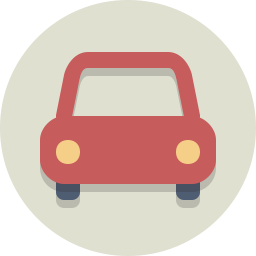
\includegraphics[width=0.5\textwidth]{logo.png}\\[1cm]
 
%----------------------------------------------------------------------------------------

%----------------------------------------------------------------------------------------
%	HEADING SECTIONS
%----------------------------------------------------------------------------------------

\textsc{\LARGE Carpool Platform}\\[1cm]

%----------------------------------------------------------------------------------------
%	TITLE SECTION
%----------------------------------------------------------------------------------------

\HRule \\[0.4cm]
{ \huge \bfseries User Manual}\\[0.4cm]
\HRule \\[1cm]
 
%----------------------------------------------------------------------------------------
%	Client SECTION
%----------------------------------------------------------------------------------------

\begin{minipage}{0.4\textwidth}
\begin{flushleft} \large
\emph{Client:}\\
Iminsys 
\end{flushleft}
\end{minipage}
~
\begin{minipage}{0.4\textwidth}
\begin{flushright} \large
\emph{Supervisor:} \\
Mr. Morkel \textsc{Theunissen}
\end{flushright}
\end{minipage}\\[1cm]

%----------------------------------------------------------------------------------------
%	Team SECTION
%----------------------------------------------------------------------------------------
\textsc{\large Team Brogrammers}\\[0.5cm]

\begin{minipage}{0.4\textwidth}
\begin{flushleft} \large
{Keagan Seddon}\\
{Leonardo Ianigro}\\
{Myron Ouyang}\\
{Marcus Bornman}\\
{Vernon Francis}\\
{Michael Yatrakos}
\end{flushleft}
\end{minipage}
~
\begin{minipage}{0.4\textwidth}
\begin{flushright} \large
\emph{u14017823} \\
\emph{u16036094} \\
\emph{u16008368} \\
\emph{u15024522} \\
\emph{u15185703} \\
\emph{u15015531} \\
\end{flushright}
\end{minipage}\\[2cm]

\vfill % Fill the rest of the page with whitespace

\end{titlepage}

\section{General Information}
\subsection{System Overview}
Carpool is a web-based platform with the goal of enabling commuters to travel together in one vehicle, as opposed to traveling alone in separate vehicles. The platform intends to achieve this goal by
connecting commuters – specifically those who travel along similar routes – and giving them the ability to plan shared commutes with each other.
\\
\\
The system allows users to create and edit profiles, add routes, communicate with other users traveling
on similar routes (based on recommendations). The system also gives users the ability to upload specific
documentation, such as driver’s licenses, to improve their security rating. Most importantly, the
platform enables users to create carpools with other users, with the intention of connecting users
traveling along similar routes and allowing them to plan routes together.
\\
\\
Finally, the system provides an intuitive trip planning interface when user’s do decide to travel together
– this interface gives users an overview of the commute, commuters, travel times, and the option to rate
other commuters when route has been completed. Giving users the ability to vouch for each other is
intended to construct an element of communal reliability between the platform community.

\subsection{System Configuration}
%System configuration image
\begin{center}
\includegraphics[width=1.0\textwidth]{configuration.png}
\end{center}
%System configuration Description
Users have access to the platform through a variety of devices with valid Internet connections, the device types include cellphones, tablets, and laptops amongst others. The configuration of the device
must allow for the use of a web browser, which is used by the user to gain access to the platform. By using the web browser, devices communicate with the web server through HTTPS, and the web server
has access to a database server through JDBC; however, this is not relevant to the user.

\subsection{Access and Installation}
The software is implemented as a progressive web application and, as such, is accessible through a web
browser on any device with an Internet connection. These are some web browsers for popular operating
systems and devices:
\begin{itemize}
\item Google Chrome, Firefox, and Internet Explorer for Windows Operating Systems.
\item Google Chrome, Firefox, and Safari for Mac Operating Systems.
\item Chrome Mobile, Firefox Mobile, and Opera Mini for Android devices.
\item Mobile Safari for iOS device.
\end{itemize}
Once accessed through a web browser, the platform can be added to device home screens or desktops
to deliver an app-like user experience. After the platform is added to a home screen or desktop is
accessible without an Internet connection but for full functionality an Internet connection is required.
The steps that need to be followed to add the platform to a device home screen are depicted below.
%Installation image
\begin{center}
\includegraphics[width=1.0\textwidth]{install.png}
\end{center}

\section{Getting Started}
\subsection{Register as a New User}
If you are accessing the platform for the very first time, you will need to register as a new user. From the landing page, click on the "Register" button. Now, fill in the details required, making sure that your details are valid and correct - the system will detect any invalid details entered and prevent you from registering. When you are satisfied that the correct details have been entered, simply click on the "Register" button to register as a new user. You can now use your email address and password to access your profile.
\begin{center}
\includegraphics[width=1.0\textwidth]{register.png}
\end{center}

\subsection{Login as an Existing User}
If you already have a registered account, you simply need to login to access your profile. From the landing page, click on the "Login" button - this will direct you to the Login Page. Now, enter your email address and the password that you chose for your account. When you are satisfied that the correct details have been entered, click on the "Login" button to access your profile.
\begin{center}
\includegraphics[width=1.0\textwidth]{login.png}
\end{center}

\subsection{Recover Forgotten Password}
If you already have a registered account, but cannot remember your password, you need to follow these steps: From the landing page, click on the "Login" button - this will direct you to the Login Page. Now, click on the text that reads "Forgot Password?". A modal will drop down asking you to input your email address - fill in the email address you registered with and submit the form. Your password will now be emailed to you and you can use it to access your account by following the instructions in section 2.2 of this manual.
\begin{center}
\includegraphics[width=1.0\textwidth]{forgot_password.png}
\end{center}

\subsection{Upload Supporting Documents}
Supporting documents, such as your ID and Driver's License, help improve your trust rating, and increase the likelihood of other users joining in a carpool with you. You can upload supporting documents from the settings page. After logging in, navigate to the settings page by clicking on the cog in the bottom left corner of the application. From the settings page, select the specific item that refers to the document you would like to upload, and click on that item. You will now be required to select the relevant file - the interface that appears here may differ depending on the device or browser you are using.
\begin{center}
\includegraphics[width=1.0\textwidth]{upload.png}
\end{center}

\subsection{Change Account Details}
If you want to change some of your account details - such as you email address or password, you can do so using the settings page. After logging in, navigate to the settings page by clicking on the cog in the bottom left corner of the application. From the settings page, select the specific item that refers to the detail you would like to change, and click on that item. Complete the relevant form and submit the change - in some cases you will have to enter the current details to before being allowed to change it, such as when changing your password.
\begin{center}
\includegraphics[width=1.0\textwidth]{edit_details.png}
\end{center}

\subsection{Logout of the Application}
It is important to note that if you are using the application from one device, you may remain logged in if you do not manually logout. To logout, navigate to the settings page by clicking on the cog in the bottom left corner of the application. On the settings page, simple select the "Log Out" option and you will be redirected to the landing page.
\begin{center}
\includegraphics[width=1.0\textwidth]{logout.png}
\end{center}

\section{Using the System}

\subsection{Creating a Route}
Your first step to traveling in a carpool is to create a route. To do this, click on the plus icon in the top right corner of the application. Now, you need to complete the route details. 
\\
\\
The route name can be anything you wish to call it - ideally, it should be descriptive of why you travel the route but it is not required as you will be the only one who can see the route name. Next, you need to enter the time that you will travel the route when you do travel the route. Then, select the days on which you will normally travel this route and finally, enter the start and end location of your route. The applications will make suggestions as you enter addresses and one of these suggestions should be selected to ensure that locations are possible to locate. 
\\
\\
When you are satisfied that all details have been completed, click on the add route button to add the route to your Home Page. You can locate the route in the "Routes" tab.
\begin{center}
\includegraphics[width=1.0\textwidth]{add_route.png}
\end{center}

\subsection{Edit or Delete an Existing Route}
To edit the details of an existing route, click on that route in the "Routes" tab on the Home Page. Then, click on the wrench located at the top right corner of the route page. You will be presented with a form which allows you to make changes to the route details. Note that any changes you make will only take effect after you click on the "Confirm Changes" button. You can also permanently delete the route by clicking on the "Delete Route" button.
\begin{center}
\includegraphics[width=1.0\textwidth]{edit_route.png}
\end{center}

\subsection{Send a Carpool Offer or Request}
Once you have created a route, you can click on that route from the home page to view people or carpools who travel along similar routes. The recommendations listed first are the ones which are best suited to you, so these are the ones you should send carpool offers or requests to first. To send a request, click on the recommendation to expand the offer modal. You can now view the route comparison between your route and the route the the recommendation is travelling - click the "Make Offer" button to send the offer or request.
\begin{center}
\includegraphics[width=1.0\textwidth]{make_route_offer.png}
\end{center}

\subsection{Respond to Offers or Requests}
You can view offers you have received from other uses in the "Carpools" tab on the Home Page. They will appear underneath the heading titled "Carpool Offers". To respond to an offer, click on the offer and select "Accept" or "Decline on the modal that appears. You also have the option of viewing the user's profile who sent the offer. If you choose to accept the offer, you will now be joined in a carpool with the user who sent the offer. 
\begin{center}
\includegraphics[width=1.0\textwidth]{offer_response.png}
\end{center}

\subsection{Make a Trip Suggestion}
Once you are joined in a carpool with other users, you have the ability to chat with them regarding possible trips, after which you can make trip suggestions. To do so, click on the carpool in the "Carpools" tab on the Home page to navigate to the chat for that carpool. After chatting to decide on a trip, the driver should make the trip suggestion by clicking on the car icon in the top right corner of the chat page. The driver will then complete the details regarding the first date and time that he intends to make the trip, on which days it will repeat following that date, and who within the carpool will be part of the trip. Once the driver is satisfied with the trip details, he/she will click on the "Suggest" button to make the suggestion.
\begin{center}
\includegraphics[width=1.0\textwidth]{make_trip_suggestion.png}
\end{center}

\subsection{Respond to Trip Suggestions}
If another member in one of your carpools has suggested a trip that includes you, you have the option to accept or decline that suggestions. To do so, click on the suggestion - this will show the details of the suggestion and give you the option to accept or decline it by clicking on the relevant button. If you choose to accept a suggestion, that trip will be added in the "Trips" tab on the Home Page.
\begin{center}
\includegraphics[width=1.0\textwidth]{accept_trip.png}
\end{center}

\subsection{View or Cancel Upcoming Trips}
You can view your upcoming trips in the "Trips" tab on the Home page. When you click on an upcoming trip, you will be presented with the details for that trip. You also have the option to cancel an upcoming trip by clicking on the the trash can in the top right corner of the trip page. Note that, unless you are the driver for that trip, canceling the trip will only remove you from the trip - other users will still partake in the trip.
\begin{center}
\includegraphics[width=1.0\textwidth]{cancel_trip.png}
\end{center}

\subsection{Review Past Trips}
After a trip has passed, you are given the opportunity to rate other users who traveled with you. These ratings will appear on each user's profile page and will be visible to all other users of the application. To review a trip, click on the past trip that you would like to review. The trip details will be displayed, but in the top right corner you can click on a star to expand a modal that gives you the opportunity to review every other user that was part of the trip. You will be required to give each user a star rate out of five and briefly describe why you gave the rating. After you are satisfied with your reviews of all the drivers, you can click on the "Submit" button. 
\begin{center}
\includegraphics[width=1.0\textwidth]{review_trip.png}
\end{center}

\subsection{View User Profiles}
Throughout the application you are given the opportunity to view user profiles - for example, when viewing the members of a carpool that you're a part of. To navigate to the user's profile page, click on the text that reads "View Profile" at any given point in the application. On  the user's profile page you can alternate between the "Vouches" and "Trust" tabs. The vouches tab lists all the reviews submitted for that user, and the trust tab indicates which documents have been uploaded by that user. Vouches in the "Vouches" tab can also be clicked on to view more details on what was said about the user.
\begin{center}
\includegraphics[width=1.0\textwidth]{view_profile.png}
\end{center}

\section{Troubleshooting}
Special efforts have been made to ensure that errors within the application are kept to a minimum; however, if the user does face any errors they should follow the instructions below.

\subsection{Form submission Errors}
Due to the nature of the platform, user's are required to fill in a substantial amount of information. If any of the information has not been entered, or entered incorrectly, the user will be faced with an error. If you face one of these errors, please review all the information you provided and ensure it is valid and accurate. The errors themselves should also provide you with an indication as to why the error is appearing.
\begin{center}
\includegraphics[width=0.3\textwidth]{form_error.png}
\end{center}

\subsection{Other Errors}
If the application produces unexpected results or errors which have not been mentioned in this manual, first attempt to refresh the page. If this is unsuccessful, log out of the application and login again. If the problem persists please notify us of the error by emailing either one of the following people:
\begin{center}
\begin{minipage}{0.4\textwidth}
\begin{flushleft}
{Keagan Seddon}\\
{Leonardo Ianigro}\\
{Myron Ouyang}\\
{Marcus Bornman}\\
{Vernon Francis}\\
{Michael Yatrakos}
\end{flushleft}
\end{minipage}
~
\begin{minipage}{0.4\textwidth}
\begin{flushright}
\emph{u14017823@tuks.co.za} \\
\emph{u16036094@tuks.co.za} \\
\emph{u16008368@tuks.co.za} \\
\emph{u15024522@tuks.co.za} \\
\emph{u15185703@tuks.co.za} \\
\emph{u15015531@tuks.co.za} \\
\end{flushright}
\end{minipage}\\
\end{center}


\end{document}